%% Microseconds Are Not the Problem -- IEEE conference version, plain-language edit.
%%
%% Hand-edited copy of manuscript-ieee.tex with the prose rewritten in a plainer, more direct
%% voice. Tables, figures, equations and every number are unchanged. This file is NOT produced
%% by scripts/make_ieee_manuscript.py; regenerating the IEEE file does not touch it.
%%
%% Build:  latexmk -pdf manuscript-ieee-plain.tex   (or two pdflatex passes)
\documentclass[conference]{IEEEtran}
\IEEEoverridecommandlockouts

\usepackage[utf8]{inputenc}
\usepackage[T1]{fontenc}

\usepackage{cite}
\usepackage{amsmath,amssymb}
\usepackage{graphicx}
\usepackage{booktabs}
\usepackage{textcomp}
\usepackage{url}
\usepackage{tikz}
\usetikzlibrary{arrows.meta, positioning, shapes.geometric}

\urlstyle{same}
\graphicspath{{figures/}}
\renewcommand{\arraystretch}{1.15}
\emergencystretch=1.5em

\begin{document}

\title{Microseconds Are Not the Problem: A Lock-Free Soft-Real-Time Data Plane for Nanopore
Adaptive Sampling, and the Signal-to-Seed Bottleneck That Bounds It}

\author{\IEEEauthorblockN{Khushal Singh}
\IEEEauthorblockA{\textit{Department of Computer Engineering} \\
\textit{National Institute of Technology Kurukshetra} \\
Kurukshetra, Haryana, India \\
khushal6002@gmail.com}
}

\maketitle

\begin{abstract}
In Oxford Nanopore adaptive sampling (``Read Until''), a client has to decide whether to eject
a molecule while it is still passing through the pore, and the decision is useless if it comes
too late. We show two things. First, speed is not the hard part. Our single-process C++20 data
plane copies signal once, passes it on without further copies, and manages buffers with a
lock-free reference-counting arena. It reaches a median per-chunk decision latency of
124.8 \textmu{}s [115.6--132.3], well under the derived service bound of 1.56 ms, and drops
nothing at genome scale. For comparison, readfish with a no-operation caller spends
124.3 \textmu{}s per read-chunk on orchestration alone on the same machine, which is the cost of
our \emph{complete} signal-space decision. Because Read Until is a soft-real-time \emph{loss
system}, a mean inside the budget says nothing about how many deadlines are missed. Second, we
find where the real limit is. At a zero-false-positive threshold our pipeline resolves
17.6\% [16.6--18.8] of reads, while RawHash2 resolves 91.8\% [91.2--92.4] of the same input. We
first modelled seed survival as $P(\mathrm{key}) = a^{E}$, with per-event bucket agreement $a$
and key length $E$, and claimed it was a lower bound. Our own measurements showed that claim
was wrong: when event retention depends on the data, $P(\mathrm{key}) \approx (1-g)^{E} a^{E}$,
where $g$ is the correspondence-failure rate. With the same estimator for both systems,
RawHash2 has $a = 0.911$, $g = 0.092$ and 467 anchors per read at $E = 8$; we have 0.783, 0.196
and 14.9 at $E = 12$. We trace this to three measured causes: the two encoders retain events
differently, our quantiser gains too little agreement, and the chainer loses anchors that could
be recovered.
\end{abstract}

\begin{IEEEkeywords}
nanopore sequencing, adaptive sampling, soft real-time systems, lock-free data structures,
raw signal mapping, quantisation
\end{IEEEkeywords}

\section{Introduction}

A nanopore sequencer reads a DNA molecule as it moves through a pore and produces an ionic
current trace in real time. Since the molecule is still inside the pore while its data comes
in, the instrument offers an interface, Read Until, through which a client can ask for an
unwanted molecule to be ejected so the channel can pick up another. The benefit is simple:
more on-target yield with the same library preparation.

The deadline here is set by physics, not by convention. Signal arrives in chunks at a fixed
rate, and each chunk describes bases that have \emph{already} gone through the pore. If the
decision arrives after the molecule has left, it is worth nothing. Suppose $C$ channels are
active, each delivering a chunk every $T_c$ seconds, and a decision is still useful up to $W$
chunks late. Then the mean service time per decision must satisfy
\[ S < \frac{W \cdot T_c}{C} \]
With $W = 2$, $C = 512$ and $T_c = 0.4$ s this is 1.5625 ms, which we round to 1.56 ms.

Two consequences shape the rest of the paper.

\textbf{It is soft real time.} A decision loses all its value at the deadline instead of
losing it gradually. So what matters is the \emph{distribution} of decision latency, not the
mean.

\textbf{It is a loss system, not a delay system.} When the client is overloaded it can either
queue work or throw it away. Queued decisions turn into late, useless ones, so dropping is the
right choice and not just a convenient one. For evaluation this means that \textbf{a mean well
inside the budget is compatible with any deadline-miss rate.} Reporting ``mean 124 \textmu{}s
against a 1.56 ms budget'' tells the reader nothing about whether deadlines are met.

Earlier Read Until work reports latency in two ways: how much signal is used before a decision
(mean bases or chunks per read), and mean processing time per read. In the systems we looked
at, we did not find a deadline-miss rate against a stated service bound, a latency distribution
with tail percentiles, or the fraction of decisions that came too late. The first half of this
paper fills that gap: we report the full distribution against a derived budget, and describe
the measurement setup in enough detail for the tail numbers to be interpretable.

\textbf{Contributions.}
\begin{enumerate}
\item A lock-free soft-real-time data plane for signal-space adaptive sampling. Its
reference-counting arena protocol rules out reset-under-dispatch by construction, without any
timing assumption (Section~\ref{sec:plane}). We evaluate it as a distribution against a derived
budget over nine runs (Section~\ref{sec:eval}).
\item A negative result with an explanation: our pipeline is $5.2\times$ less accurate than a
published signal-space mapper on the same input, and we show that the cause lies before seeding
(Section~\ref{sec:gap}).
\item A seed-survival law, including the correction of our own earlier version of it, and a
measurement of its two parameters for both systems using the same estimator
(Section~\ref{sec:law}).
\item Three measured root causes and what they imply for design (Section~\ref{sec:causes}).
\end{enumerate}

\textbf{What we do not claim.} We do not claim competitive mapping accuracy; we report 17.6\%
against 91.8\% and explain why. We do not claim a new matching method; quantised-event hashing
already exists~\cite{rawhash,rawhash2}. We do not claim reliable tail latency, because every
measurement was taken under a hypervisor; Section~\ref{sec:limits} explains what that allows us
to say. All signal is simulated.

\section{Background and related work}

\textbf{The interface.} MinKNOW~\cite{minknow} provides a bidirectional streaming RPC that sends
raw signal chunks for each channel and accepts actions back. Reads are identified by a string;
version 6.0 removed the numeric read index from the API, which affects how client-side data
structures can be built.

\textbf{Basecalling clients.} readfish~\cite{readfish} and similar tools basecall each chunk and
then map the resulting sequence. This is accurate and reuses well-tested software, but it puts a
neural network and a sequence aligner~\cite{minimap2} inside the decision loop.

\textbf{Signal-space mappers} skip basecalling. They convert the reference into expected signal
using a pore model and match quantised query events against it directly. UNCALLED~\cite{uncalled}
uses an FM-index over events; Sigmap~\cite{sigmap} and RawHash~\cite{rawhash} seed and chain
over quantised event $k$-mers; RawHash2~\cite{rawhash2} adds an adaptive quantiser;
RawAlign~\cite{rawalign} adds alignment after seeding; Sigmoni~\cite{sigmoni} classifies reads
with an $r$-index over a small picoamp alphabet. The RawBench framework~\cite{rawbench} splits
raw signal analysis into reference encoding, segmentation and matching, and compares three
segmentation methods: t-test changepoint detection, basecaller move tables, and a learned
segmenter. We use the same split, and further divide matching into quantisation, seeding and
chaining, because our analysis needs that level of detail.

\textbf{The stages run in order, and each one limits the next.} Reference encoding
$\rightarrow$ segmentation $\rightarrow$ quantisation $\rightarrow$ seeding $\rightarrow$
chaining. Chaining cannot recover information that quantisation has already thrown away.
Sections~\ref{sec:gap}--\ref{sec:causes} are built on this point.

\textbf{Streaming decision structures.} Misra--Gries~\cite{misragries} and
Space-Saving~\cite{spacesaving} track approximately frequent items in bounded memory. We use a
set-associative variant whose update costs $O(\text{ways})$ instead of $O(\text{counters})$,
which matters on the decision path.

\textbf{Simulation.} Squigulator~\cite{squigulator} generates signal with adjustable dwell-time
variation; by default the coefficient of variation is about 0.44. Icarust~\cite{icarust} serves a
live Read Until API but emits a fixed number of samples per $k$-mer, which is exactly the CV $= 0$
case. We patched it to draw dwell times from a lognormal distribution.

\section{The data plane}
\label{sec:plane}

\subsection{Design constraints}

The design follows four rules. The decision path must not allocate memory, since an allocator
can take an unbounded amount of time. It must not take a lock, since a blocked worker will miss
its deadline. State must be $O(\text{channels})$ with fixed per-channel sizes known at compile
time, because read length depends on library preparation and cannot be known in advance.
Finally, under backpressure the system must drop work rather than queue it, for the loss-system
reason given in Section~I.

\subsection{Single-copy ingestion, zero-copy propagation}

Signal is copied exactly once, when the protobuf runtime writes it into arena-backed storage at
the transport boundary. Nothing after that copies it again. Workers get a 56-byte borrowed
descriptor containing an absolute sample index, pointers into the arena-owned read-identifier
and payload storage, the arena slot that owns them, a receive timestamp, and a few lengths and
type codes. With fields in the obvious order the structure is 72 bytes; reordered for size it is
56. We noticed the difference because a compile-time check that it fits in one cacheline failed.

Two fields are narrowed, with checks at ingest. Chunk length goes from 64 to 32 bits, since a
chunk is under a second long and $2^{32}$ samples is about twelve days at 4 kHz. Read-identifier
length goes to 16 bits, since identifiers are 36-character UUIDs. We deliberately do \emph{not}
narrow the absolute sample index: a 72-hour run at 4 kHz already reaches ${\approx}10^9$, which
is too close to $2^{32}$.

\subsection{The arena reference-counting protocol}

The danger is reset-under-dispatch: an arena slot gets reused while a descriptor pointing into
it is still sitting in a ring. The memory stays mapped and owned by the arena, so this does not
crash; it silently corrupts the payload.

The protocol prevents it by design (Figure~\ref{fig:arena}). \texttt{acquire()} returns a slot
with refcount 1, and that first reference belongs to the \textbf{reader}, not to any consumer.
The reader pushes descriptors to $n$ shard rings, which raises the count to $1 + n$, and only
then drops its own reference. So the count can only reach zero after every worker has taken and
released its reference, and a slot cannot be reset while any dispatch is still pending. This
holds no matter how long a worker takes.

\begin{figure}[t]
\centering
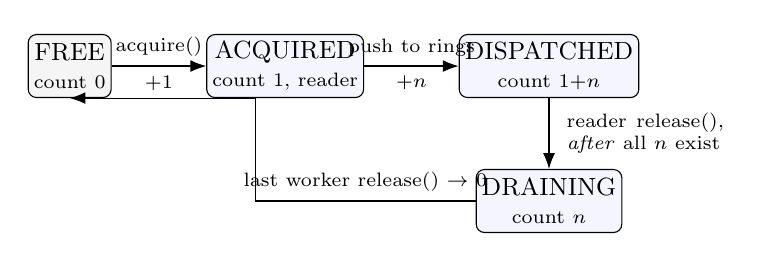
\begin{tikzpicture}[
  node distance=5mm,
  state/.style={draw, rounded corners=3pt, align=center, font=\small,
                minimum height=8mm, inner sep=2pt, fill=blue!4},
  free/.style={state, fill=black!4},
  lbl/.style={font=\scriptsize, align=center}]
\node[free] (f) {FREE\\[-1pt]\scriptsize count 0};
\node[state, right=12mm of f] (a) {ACQUIRED\\[-1pt]\scriptsize count 1, reader};
\node[state, right=12mm of a] (d) {DISPATCHED\\[-1pt]\scriptsize count $1{+}n$};
\node[state, below=9mm of d] (r) {DRAINING\\[-1pt]\scriptsize count $n$};
\draw[-{Latex[length=2mm]}] (f) -- node[lbl, above]{acquire()} node[lbl,below]{$+1$} (a);
\draw[-{Latex[length=2mm]}] (a) -- node[lbl, above]{push to rings} node[lbl,below]{$+n$} (d);
\draw[-{Latex[length=2mm]}] (d) -- node[lbl, right, xshift=1mm]{\parbox{20mm}{reader
  release(), \emph{after} all $n$ exist}} (r);
\draw[-{Latex[length=2mm]}] (r.west) -- ++(-28mm,0) node[lbl, above, midway]
  {last worker release() $\rightarrow$ 0} |- (f.south);
\end{tikzpicture}
\caption{Lifetime of an arena slot. Because the reader holds the first reference, the count
cannot reach zero while a descriptor is still in a ring, whatever the worker timing.}
\label{fig:arena}
\end{figure}

\subsection{Lock-free handoff and sharding}

Threads hand off work through single-producer single-consumer rings. The rings use free-running
64-bit counters and power-of-two capacity, so indexing is a mask instead of a modulus and every
slot can be used, not just capacity $-\,1$. Producer and consumer each keep a cached copy of the
other's index, which avoids cross-core loads when the ring is not full; head, tail and both
cached copies sit on separate cachelines. Shard rings hold 2048 descriptors and action rings
hold 1024. With four shards the rings take under 0.75 MB in total, which is small next to the
index.

Chunks are assigned to shards by \texttt{channel \& mask}, so each channel's state is touched by
exactly one thread \textbf{by construction}. That is why the lock-free design is cheap: there is
no shared, mutable per-channel state to protect. Under backpressure we drop and never block, and
counters maintain the invariant $\textit{offered} = \textit{pushed} + \textit{dropped}$.

\subsection{Bounded per-channel state}

Most of the per-channel state is the decision structure. The set-associative vote table takes
$64 \times 4 \times 12$ B $=$ 3,072 B per channel (1.57 MB at 512 channels, 8.22 MB at 2675).
An update costs $O(4)$, where a classical Misra--Gries table with the same number of counters
would cost $O(256)$; its expected retention threshold is $m/320$ against $m/257$. The
anchor-history chainer takes $1024 \times 14$ B $=$ 14,336 B per channel. Each of these is a
compile-time constant multiplied by the number of channels; none depends on read length or on
how long the run has been going.

\subsection{Thread topology}

We place threads using the kernel's SMT sibling sets instead of computing processor indices.
This matters in practice. Our test machine lists siblings next to each other
(\texttt{0-1 2-3 4-5 6-7}), so an earlier rule that gave each role ``the next logical
processor'' put the reader and writer on \emph{the same physical core} and left two cores
unused. The numbering differs between machines. With two shards the data plane uses four
threads (reader, writer, two workers), which fit on four physical cores; with four shards it
uses six, which do not.

\section{Evaluation of the data plane}
\label{sec:eval}

\subsection{Method and instrumentation}

We measure latency from the moment the transport read returns to the moment the decision is
made, and record it with HdrHistogram~\cite{hdrhistogram} at three significant figures, which
keeps relative error within 0.1\%. Every output line names the recording backend, so a fallback
estimate cannot be confused with a real measurement.

We changed instruments for a reason. An earlier power-of-two histogram gave 99th percentiles of
111.93, 112.12, 223.66 and 447.59 \textmu{}s over four runs. At the host's calibrated invariant
TSC frequency of 2418.7 MHz, the only values it could represent in that range were 54.19,
108.38, 216.76 and 433.53 \textmu{}s. Every reported value was a bucket edge, so two runs that
``agreed'' at 112 \textmu{}s only agreed that the true value was somewhere in [54.19, 108.38].
More generally, \emph{any} instrument whose resolution is coarse compared with the run-to-run
variation will show stable numbers and make the system look more stable than it is.

For every run the harness records virtualisation status, SMT topology, TSC flags,
clocksource, kernel command line, governor, turbo state, free storage and load average. It only
marks a run as publishable if there is no virtualisation, cores are isolated and the governor is
set to performance. All runs in this paper are marked development-only.

\textbf{Host.} Intel Core i5-1135G7, 4 physical cores / 8 logical, under WSL2.
\textbf{Regimes.} R1: a 37 kb reference with constant dwell. R3: a 64 Mb human chr20 reference
with variable dwell, using the frozen configuration: 4 bits $\times$ 12 events,
minimizer~\cite{minimizers} window 1, detected-event segmentation, two shards, pinned.

\subsection{Placement and thread count}

\begin{table}[t]
\caption{Regime R1, 37 kb reference, four repetitions per cell. Median across runs, \textmu{}s.}
\label{tab:r1}
\centering
\footnotesize
\begin{tabular}{lrrrr}
\toprule
configuration & p50 & p90 & p99 & p99.9 \\
\midrule
pinned, 2 shards   & 16.3 & 24.7 & 49.1 & 158.0 \\
unpinned, 2 shards & 15.8 & 25.1 & 50.5 & 165.7 \\
pinned, 4 shards   & 18.7 & 31.1 & 70.4 & 312.7 \\
unpinned, 4 shards & 18.4 & 31.6 & 83.8 & 386.7 \\
\bottomrule
\end{tabular}
\end{table}

\textbf{Thread count matters more than placement.} Both two-shard settings beat both four-shard
settings at every percentile (Table~\ref{tab:r1}), because six data-plane threads do not fit on
four physical cores.

\textbf{Pinning does not lower the median, but it makes the tail repeatable.} Over four
repetitions the 99th percentile is 46.99, 48.32, 49.97, 50.88 \textmu{}s when pinned (a spread of
8\%) and 44.86, 45.52, 55.45, 104.45 \textmu{}s when unpinned (a spread of 133\%). So the honest
claim about processor affinity concerns variance, not the typical value.

\subsection{Genome scale: regime R3}

We ran nine 40 s runs. In every log the daemon's startup line confirms the configuration:
63,981,237 reference bases, geometry $4 \times 12 = 48$-bit keys, window 1, 63,981,218
minimizers, 32,888,127 distinct keys, 512.0 MiB table + 204.3 MiB positions.

\begin{table}[t]
\caption{Regime R3, nine runs. Median across runs, with observed range, \textmu{}s.}
\label{tab:r3}
\centering
\footnotesize
\begin{tabular}{lr}
\toprule
percentile & median [range] \\
\midrule
p50   & 124.8 [115.6--132.3] \\
p90   & 192.8 [183.0--306.0] \\
p99   & 370.2 [346.8--1969.3] \\
p99.9 & 1224.5 [1044.9--3284.0] \\
mean  & 138.2 [131.2--206.0] \\
\bottomrule
\end{tabular}
\end{table}

Peak resident set is 3.70 GiB in every run. That figure includes the temporary memory used while
building the index; the index structures in steady state take 716 MiB. Chunks arrive at
604--645 per second, a rate set by the simulator and not by the daemon. \textbf{No chunks were
dropped and no deadline misses were recorded in any of the nine runs.}

At the median, utilisation is \textbf{0.080} of the 1.56 ms bound. A 10-chunk read finishes its
decisions in \textbf{1.25 ms}. This is calculated (ten chunks times the measured median per-chunk
latency), not measured separately.

\textbf{The tail is where the loss-system view matters.} Eight of the nine runs stay inside the
budget up to the 99.9th percentile, at 1.04--1.40 ms. The ninth does not: it reports
p99 $=$ 1969.3 \textmu{}s and p99.9 $=$ 3284.0 \textmu{}s, and it is also the worst run at p90 and
at the mean (Figure~\ref{fig:r3}).

We do not treat this as a real deadline miss. Across the nine runs the observed \emph{maximum}
ranges from 2.0 ms to 59.4 ms, a factor of about a hundred in a quantity the software itself
should not vary in. Also, the run with the largest maximum is \textbf{not} the one with the worst
p99; its p99 is 630 \textmu{}s. When maximum and p99 do not move together like this, the likely
cause is stalls coming from outside the program, not slow decisions. On a hypervisor without
isolated cores, this data cannot show that the system meets its deadline, and it cannot show
that it misses it either. We think it is important to say so plainly.

\begin{figure*}[t]
\centering
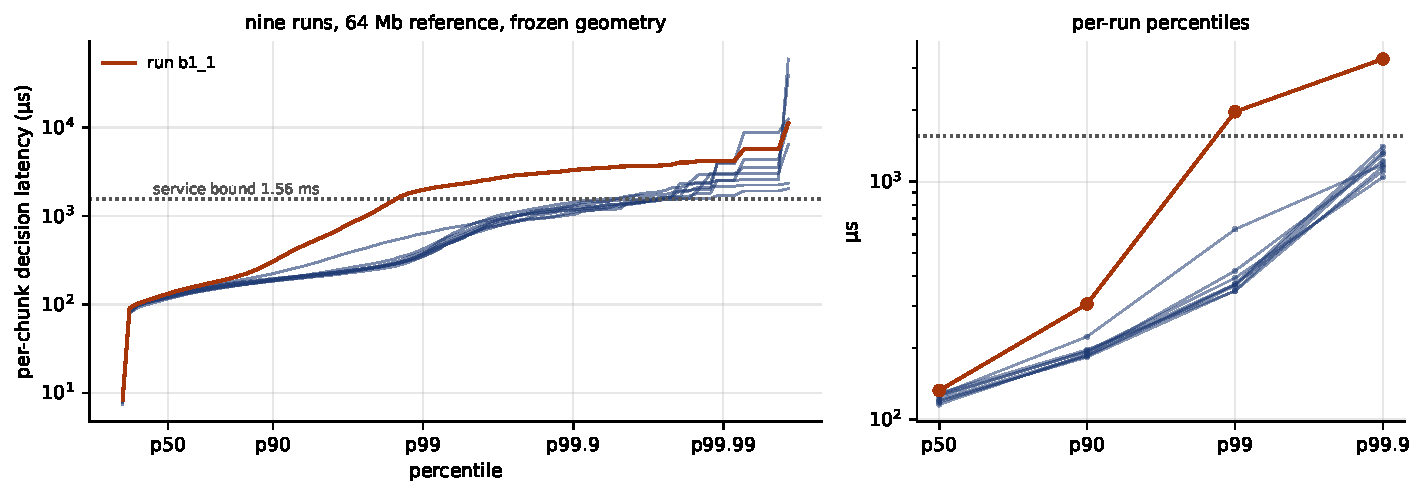
\includegraphics[width=0.86\textwidth]{fig5-4-r3-distribution.pdf}
\caption{Regime R3 over nine runs, against the 1.56 ms service bound. Eight runs stay inside the
budget up to p99.9; one goes over at p99 and p99.9.}
\label{fig:r3}
\end{figure*}

\subsection{Comparison with existing clients}

\begin{table}[t]
\caption{Cost comparison on the same host. readfish figures are its own progress line divided
out; processor and memory figures are from \texttt{/usr/bin/time -v}.}
\label{tab:costs}
\centering
\scriptsize
\begin{tabular}{llrrr}
\toprule
system & mode & per chunk & CPU & peak RSS \\
\midrule
readfish  & no-op caller      & 124.3 \textmu{}s & 15.6\%  & 86.0 MiB \\
readfish  & caller + mapper   & 66.2 \textmu{}s  & 25.3\%  & 663.4 MiB \\
this work & frozen, 64 Mb     & 124.8 \textmu{}s & 181.5--202.3\% & 3786 MiB \\
\bottomrule
\end{tabular}
\end{table}

\textbf{What the comparison shows.} With a no-operation caller, readfish does no basecalling and
no mapping, so its 124.3 \textmu{}s is pure orchestration and a lower bound on its cost. Our
\emph{complete} signal-space decision over a 64 Mb index takes 124.8 \textmu{}s. In other words,
the orchestration layer of a basecalling client already costs as much as an entire signal-space
decision. This does not mean our system is better, since a production readfish does work that
this configuration leaves out. It does mean that the time budget is not what is holding
signal-space matching back.

The price is processor time: 181.5--202.3\% of one core, against 15.6\% for readfish, because
our workers spin before they yield. We report this next to the latency.

\textbf{Against a signal-space mapper.} Run single-threaded on the same reads with the same pore
model, RawHash2 needs 10.64 ms of processor time per read including index loading, or 10.18 ms
without it (a long-running daemon loads the index only once). Our comparable figure is the
derived 1.25 ms. That is a ratio of $8.2\times$, but it has to be read together with
Section~\ref{sec:gap}: comparing the speed of a system that resolves most reads with one that
mostly does not only bounds the data-plane cost. It is not a performance result.

\section{The accuracy gap}
\label{sec:gap}

\subsection{Head-to-head}

We ran both systems on the same 20 Mb chr20 reference, with the same Squigulator-derived R10.4
9-mer pore model on both sides, the same SLOW5 files, three seeds and 500 reads per cell, at
Squigulator's default dwell variation.

For our system we report the true-positive rate at the lowest threshold that gives zero false
positives on a shuffled control with matched composition. For RawHash2 we report the fraction
mapped correctly at its own default operating point, which is \textbf{not} zero-false-positive:
it maps 8.4--10.6\% of control reads. So the comparison is about size of effect, not exact
level, and we present it that way.

\begin{table}[t]
\caption{Accuracy, three seeds, 500 reads per cell.}
\label{tab:acc}
\centering
\footnotesize
\begin{tabular}{lrrrr}
\toprule
system & s42 & s43 & s44 & mean [range] \\
\midrule
this work  & 18.8 & 17.4 & 16.6 & \textbf{17.6} [16.6--18.8] \\
RawHash2   & 92.4 & 91.8 & 91.2 & \textbf{91.8} [91.2--92.4] \\
\bottomrule
\end{tabular}
\end{table}

The difference is a factor of 5.2 (Table~\ref{tab:acc}). The rest of the paper explains where it
comes from.

\subsection{Replication is necessary at this scale}

\begin{table}[t]
\caption{Decision rules at the same operating point, three seeds.}
\label{tab:rules}
\centering
\scriptsize
\begin{tabular}{lrrrr}
\toprule
decision rule & s42 & s43 & s44 & mean [range] \\
\midrule
votes (256 counters)        & 14.2 & 15.0 & 13.0 & 14.1 [13.0--15.0] \\
greedy, $\beta = 0$ (ctrl)  & 9.6 & 10.8 & 7.0 & 9.1 [7.0--10.8] \\
greedy, $\beta = 12$        & 17.4 & 16.6 & 15.6 & 16.5 [15.6--17.4] \\
anchor-history, $L = 48$    & 18.8 & 17.4 & 16.6 & 17.6 [16.6--18.8] \\
anchor-history, $L = 128$   & 19.6 & 19.4 & 18.0 & \textbf{19.0} [18.0--19.6] \\
\quad $L = 48$, occ. filter & 17.8 & 15.8 & 15.4 & 16.3 [15.4--17.8] \\
\bottomrule
\end{tabular}
\end{table}

Table~\ref{tab:rules} lists six decision rules, each run with three seeds.

\textbf{The $\beta = 0$ control tells us the most.} Without gap tolerance, chaining does
\emph{worse} than the vote table (9.1\% against 14.1\%), which is what we would expect since it
follows 24 candidates while the table follows 256. So the gain comes from the gap tolerance, not
from switching data structures.

\textbf{The best rule improves on voting by $+35\%$ relative}, 19.0\% against 14.1\%. Nothing we
tried did better.

\textbf{A single rule can vary by up to 3.8 points between seeds.} The control alone goes from
7.0 to 10.8. That is about as large as the differences \emph{between} rules, and neighbouring
rules have overlapping ranges. Any two configurations less than about four points apart need
repeated runs to compare. We found this out the hard way: an earlier single-run table said that
raising look-back from 48 to 128 did not help. It does help, by 1.4 points on average and in
every seed. The single run behind the old claim had used a different seed from the other five
rows of that table.

Even the best decision rule changes accuracy by tens of percent, while the gap is a factor of
five. The problem is not in the decision rule.

\section{A seed-survival law}
\label{sec:law}

\subsection{The model, and why our original bound was wrong}

Let $a$ be the probability that the reference and the query put corresponding events in the
same quantiser bucket. A key is made of $E$ consecutive events, so it matches only if all $E$
agree, and the expected number of anchors falls like $a^{E}$.

At first we argued that this was a \textbf{lower} bound. Two effects make per-event agreements
positively correlated. Neighbouring events come from overlapping $k$-mers (adjacent 9-mers share
eight bases), and all events in a read are normalised with one shift-and-scale estimate, so an
error in that estimate moves all of the read's $z$-values together. With positive correlation,
agreements come in clusters, which makes a full run of $E$ agreements more likely than if events
were independent.

\textbf{That argument only works under a condition, and for most configurations we care about
the condition does not hold.} It assumes the two event sequences line up exactly. If a key
window contains even one inserted or deleted event, it cannot match, however well the other
events agree. Let $g$ be the probability that an alignment column is an indel instead of a
matched pair. Then
\[ P(\mathrm{key}) \approx (1-g)^{E} \cdot a^{E} \]
and the simple form leaves out the first factor. When segmentation is fixed-width and dwell is
constant, $g$ is small and $a^{E}$ does act as the lower bound argued above; in the two such
configurations it is $1.8\times$ and $5.1\times$ below the direct count. When segmentation
depends on the data or dwell varies, $g$ goes up to 0.09--0.21 and $a^{E}$ becomes an
\textbf{over-estimate}, by $1.9\times$ to $14\times$ across the other cells
(Figure~\ref{fig:modelmeas}).

The main idea still holds: yield drops geometrically with $E$, and the base of that drop is a
measurable property of the quantiser. But $a^{E}$ can only be used as a one-sided bound when the
correspondence is exact.

\subsection{Measuring both systems the same way}

Agreement numbers computed differently for two systems cannot be compared. So we export the
per-event quantised symbols of both systems in a single format and score them with a single
program, which does not know which system the input came from.

Our symbols come from the same reference-encoding and quantisation code used in production.
RawHash2 has an \texttt{--out-quantize} option that dumps query-side symbols, but its reference
path has the dump switched off in the code. We added a four-line \texttt{--out-quantize-ref}
option that does the same on the reference side, and fixed a record-separator bug that made the
standard multi-read output impossible to parse.

The scorer aligns the two symbol streams semi-globally (the query is aligned end to end, end
gaps on the reference are free, match $+1$, mismatch $-1$, gap $-1$). It reports $a$ under the
best alignment, $a$ under the best single constant offset, the indel fraction, and, read directly
off the alignment path, the fraction of positions that start an unbroken run of $E$ matching
columns. That last number is $P(\mathrm{key})$ \textbf{measured, not modelled}, so no
independence assumption is needed at all.

\textbf{Validation.} Under the same conditions as our earlier per-event diagnostic, the new
instrument gives a constant-offset agreement of 0.556, against the 0.559 reported before:
different code on the same input, agreeing within 0.3 percentage points.

\textbf{Choice of estimator.} The constant-offset estimator, which we used in earlier work,
underestimates agreement by about four times once retention depends on the data: 0.188 for our
frozen configuration, where the correspondence-aware value is 0.783. We withdraw the results we
obtained with it for detected-event configurations, including the claim that detection roughly
halves agreement. It does not.

\subsection{Results}

\begin{table}[t]
\caption{Agreement, correspondence failure, and measured key-match probability. 200 reads per
cell, identical input, one estimator.}
\label{tab:agree}
\centering
\scriptsize
\begin{tabular}{llrrrrr}
\toprule
system & CV & $a$ & $g$ & $E$ & $P(\mathrm{key})$ & anchors \\
\midrule
this work & 0.00 & 0.797 & 0.170 & 12 & 0.0124 & 33.8 \\
this work & 0.44 & 0.783 & 0.196 & 12 & 0.0055 & 14.9 \\
RawHash2  & 0.00 & 0.913 & 0.055 & 8  & 0.350  & 651 \\
RawHash2  & 0.44 & 0.911 & 0.092 & 8  & 0.254  & 467 \\
\bottomrule
\end{tabular}
\end{table}

\textbf{The gap is large, and it appears before seeding.} At CV 0.44 the measured key-match
probability differs by a factor of \textbf{46} (0.254 against 0.0055), and the number of anchors
by a factor of \textbf{31} (467 against 14.9 per read). The two ratios differ because the systems
keep different numbers of events per read (Table~\ref{tab:agree}). A 31-fold difference in
anchors is enough to explain 91.8\% against 17.6\% without looking at the decision rule at all.

\textbf{The key-match difference can be split, and key length is the smaller part.} In our own
pipeline, measured $P(\mathrm{key})$ at $E = 8$ instead of 12 is 0.0274 against 0.0055, a factor
of \textbf{4.9}. The remaining factor of \textbf{9.3} (0.254 against 0.0274 at the same key
length) comes from the encoding and segmentation themselves ($4.9 \times 9.3 = 45.8$, which gives
back the 46-fold total). So shortening keys is the smaller lever, and, as
Section~\ref{sec:causes} shows, its gain is cancelled by lost specificity.

\textbf{RawHash2's agreement does not change with dwell; ours does.} Between CV 0 and 0.44 it
moves 0.913 $\rightarrow$ 0.911, while ours moves 0.797 $\rightarrow$ 0.783. Over the same
range our key-match probability drops $2.2\times$, because $g$ rises from 0.170 to 0.196. It is
correspondence that changes, not agreement.

\begin{figure*}[t]
\centering
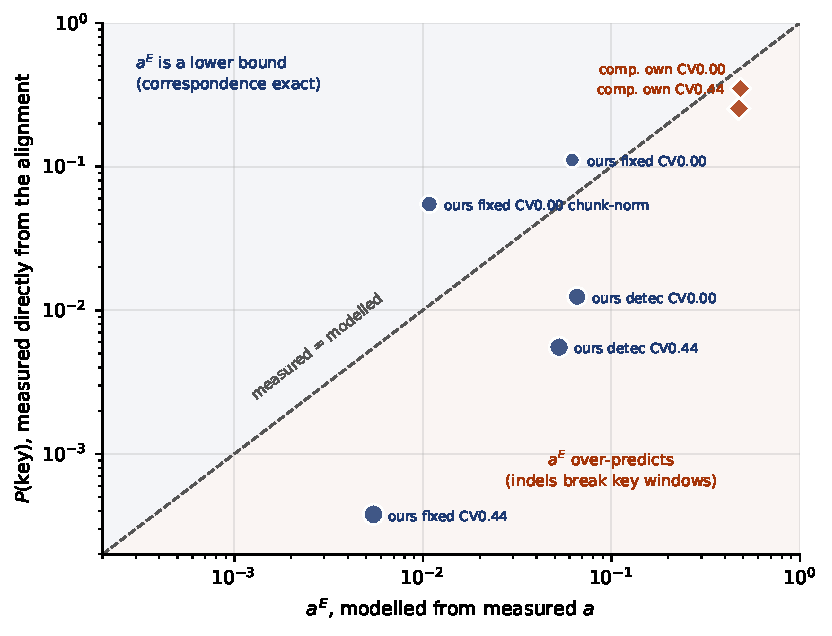
\includegraphics[width=0.70\textwidth]{fig7-3-model-vs-measured.pdf}
\caption{Measured key-match probability against the $a^{E}$ prediction. Marker area shows the
correspondence-failure rate $g$. $a^{E}$ is a lower bound only when correspondence is exact.}
\label{fig:modelmeas}
\end{figure*}

\section{Three root causes}
\label{sec:causes}

\subsection{Asymmetric event retention}

RawHash2 merges events with one rule: drop any event whose level is within
\texttt{--sig-diff} $=$ 0.35 of the last kept event. It applies this rule \textbf{in the same way
to the reference encoding and to the query}, and keeps 73.4\% of events on each side. As a
result both sides agree on how many events a given stretch of sequence contains.

Our pipeline does not do this. The reference encoder produces one event per $k$-mer, always,
while the query detector produces about 0.78. The effect is easy to see: our indel rate is
\textbf{0.170 at zero dwell variation}, where there is no timing noise at all. An indel rate that
high without noise comes from a mismatch between the two encoders, not from the signal. Since
correspondence failure has the same exponent in $P(\mathrm{key})$ as disagreement, it costs just
as much. This is the first thing to fix, and it is a change to the indexing code, not an open
research problem.

\subsection{A ${\approx}2.5$-bit quantisation sweet spot}

RawHash2 nominally uses four bits, which allows sixteen buckets. On chr20 its symbols actually
fall into six of them (7.7, 21.1, 9.7, 27.6, 24.0 and 8.8 per cent, plus a 0.9 per cent outlier
bucket), giving a realised entropy of about \textbf{2.46 bits per event}. The quantiser is
non-uniform on purpose: fine steps in a central band and coarse steps outside it.

A third system points to the same place, which makes coincidence less likely.
Sigmoni~\cite{sigmoni} classifies instead of mapping and shares none of our decision code, yet
by default it quantises into \textbf{six} symbols (2.58 bits). Its authors say this balances
robustness to noise against specificity in exact matching. Two independent systems ending up
within a tenth of a bit of each other, one of them citing noise robustness as the reason,
suggests that this operating point is a real one.

Our uniform quantiser over a clipped $z$-range spreads values evenly across its alphabet, uses
more of it, and agrees less often. \textbf{The trade-off is per-event entropy against per-event
agreement, and the two systems sit at opposite ends of it.} An 8-event key at 2.46 bits holds
about 19.7 bits of nominal specificity; a 12-event key at nearly 4 realised bits holds about 48.
Yet the system with the \emph{less} specific key is five times more accurate. Specificity beyond
what it needs costs it nothing, while the agreement we lack costs us almost everything.

\textbf{Encoding differences does not help, and the reason is useful.} If we encode the
\emph{difference} between successive levels, the shared per-read normalisation shift cancels
out. Measured over three seeds, though, it does much worse: 8.3 [3.6--11.8] against 17.6 for the
absolute encoding, and worse in every seed. It still used one symbol per event and only changed
what the symbol meant. So $E$ agreements were still needed, and each symbol now depended on two
noisy levels instead of one. It went after the right quantity in the wrong way. Merging instead
lowers $E$ \emph{and} raises $a$, and the $(1-g)^{E} a^{E}$ form rewards both.

\begin{table}[t]
\caption{Realised key entropy and occurrence-cap survival, 20 Mb reference.}
\label{tab:entropy}
\centering
\scriptsize
\begin{tabular}{lrrrrr}
\toprule
geometry & nominal & distinct keys & realised & short & cap \\
\midrule
$3 \times 8$  & 24 & 92,482     & 16.5 & 7.5  & 2.8\%  \\
$4 \times 8$  & 32 & 1,519,844  & 20.5 & 11.5 & 31.2\% \\
$3 \times 13$ & 39 & 5,096,781  & 22.3 & 16.7 & 63.7\% \\
$3 \times 14$ & 42 & 7,985,629  & 22.9 & 19.1 & 78.8\% \\
$4 \times 12$ & 48 & 14,908,778 & 23.8 & 24.2 & 93.5\% \\
\bottomrule
\end{tabular}
\end{table}

\textbf{Specificity also depends on scale.} A 39-bit key realises 22.3 bits, 16.7 short of
nominal; the frozen 48-bit key realises 23.8, 24.2 short (Table~\ref{tab:entropy}). \textbf{The
shortfall grows faster than the nominal width}: doubling the nominal key space from 24 to 48
bits adds only 7.3 bits of realised entropy.

Short keys hit the occurrence cap, and more so on larger references. A $3 \times 8$ geometry
keeps only 2.8\% of minimizer occurrences on the 20 Mb reference (97.2\% truncated), and 0.7\% on
the 64 Mb one (99.3\% truncated). Short keys get worse faster than the reference grows, so a
geometry tuned on a small reference does not carry over to a large one. This is why shortening
keys to get more anchors does not work: realised entropy collapses before the extra anchors
become useful.

\subsection{Recoverable loss inside the chainer}

With the correspondence-aware measurement, the anchor supply of our frozen configuration
changes from a modelled 1.85 per read (from the simple $a^{E}$ form, for a \emph{fixed-width}
configuration we do not use) to a measured \textbf{14.9} for the configuration we actually use.
The observed median best-chain score is \textbf{4}.

So about 11 of the 15 anchor-eligible positions in a read do not make it into the best chain. We
could not see this loss while the estimate was \emph{below} the observed score: a decision stage
cannot find more anchors than exist, and 1.85 against 4 left no room for any loss. Possible
causes are the occurrence cap discarding anchors before chaining, the 24-slot greedy chainer
thrashing, and a chaining band of 12 against a measured indel rate of 0.196. We have not yet
worked out which one it is.

This adds to, but does not change, our conclusion about where the main problem is. Closing a
31-fold gap in anchor supply matters more than recovering a factor of less than four. Still, the
decision stage is not entirely innocent, and since we know the anchors are there, finding the
loss is a matter of diagnosis rather than search.

\section{Discussion}
\textbf{Measure $a$ and $g$ before designing a decision rule.} Each takes one pass over paired
reference and query events, with no training and no search, and together they tell you whether
\emph{any} decision rule can work before you build one. A paper that reports a decision rule
without agreement and correspondence figures does not give readers enough to judge it.
\textbf{Optimise key-match probability, not agreement alone}: correspondence failure has the same
exponent as disagreement, and our indel rate is 0.170 even with no timing noise. What you trade
to improve both is alphabet size, which RawHash2 and Sigmoni give up and we hold on to.

\textbf{Report distributions against derived budgets}, since under a deadline a mean inside the
budget fits any miss rate; we give nine runs with full ranges and point out the one that goes
over. And \textbf{run the external baseline first, not last}. We measured every change to the
decision stage against our own earlier results. Those numbers went up and down in believable
ways and never hinted that the real limit was somewhere else. A single run of a published tool on
the same input would have shown within a day that the gap was a factor of five, not a matter of
tuning. When pipeline stages run in order, a series of internal improvements is measured against
the wrong baseline until an outside reference sets the scale.

\section{Limitations and threats to validity}
\label{sec:limits}

\textbf{All latency figures were measured under a hypervisor.} WSL2 can pause a vCPU in the
middle of a decision, and in the data that looks the same as a slow decision. We treat p50 and
p90 as properties of our implementation, and p99 and above as upper bounds affected by the
platform. The 2.0--59.4 ms spread of observed maxima, which does not track p99, is the direct
evidence for this. Measuring a deadline-miss rate against the 1.56 ms bound needs bare metal
with isolated cores, tickless operation, interrupts moved off the measured cores and a fixed
governor. We did not have such a machine, and none of our claims depend on the tail.

\textbf{All signal is simulated.} It comes from two generators whose detector calibrations differ
by a factor of thirty, and every result uses a single reference, human chr20. Agreement is
measured at two dwell levels, with one seed and 200 reads per cell, whereas accuracy is measured
at six levels with three seeds; so the claim that RawHash2's agreement does not depend on dwell
rests on two points. The alignment-based agreement figures are upper bounds, since they use the
correspondence that gives the most matches. Indel fractions of 0.055--0.208 mean the alignments
stay close to the diagonal, so the estimator is not creating matches through heavy gapping, but
the bound is still one-sided and the bias favours RawHash2. The symmetric-retention explanation
can be seen in RawHash2's source and fits every measurement, but we have not run the deciding
experiment: applying our detector to our own reference encoding and measuring again. We built and
ran RawHash2, Squigulator, readfish and Icarust ourselves; what we say about UNCALLED, Sigmap,
RawAlign and Sigmoni is based on their papers and repositories, not on running them.

\section{Conclusion}

We asked whether the adaptive-sampling decision can be made in microseconds. It can: the median
is 124.8 \textmu{}s at genome scale against a 1.56 ms physical budget, with bounded per-channel
state, no allocation on the decision path and no drops at the offered rate. The orchestration
layer of a standard basecalling client alone costs 124.3 \textmu{}s per read-chunk before it makes
any decision. Time is not what blocks signal-space adaptive sampling.

The more useful finding is why speed is not enough. Quantised-event matching is limited not by
how fast decisions can be made but by how well the signal survives segmentation and
quantisation. Two measurable quantities capture this, and their product raised to the power $E$
controls everything after them. At the agreement and correspondence our pipeline reaches, no
decision rule placed after quantisation can recover what segmentation and quantisation have lost.
That is why six different attempts at the decision rule changed accuracy by at most 35\%
relative, while the gap was a factor of five.

This is a negative result for our system and a pointer to where improvement has to come from. A
system whose failure is measured, modelled and shown to explain why six fixes did not work is
more useful to the next designer than one that works for reasons nobody can explain.

\section*{Reproducibility}

All code, data and scripts are in the accompanying repository at commit \texttt{eb0ea28}.
\texttt{scripts/verify\_thesis\_numbers.py} recomputes every number from the files under
\texttt{results/}. For figures that describe code which no longer exists, it checks them against
the commit message that recorded them. It exits with an error on any mismatch, and currently
reports 143 claims agreeing and none disagreeing. \texttt{scripts/verify\_paper\_numbers.py}
runs the same check on this manuscript. \texttt{scripts/generate\_thesis\_figures.py} rebuilds
every data figure from \texttt{results/} alone, byte for byte. Five claims are not covered by any
committed file and are listed as scope limits: a bare-metal deadline-miss rate, real instrument
data, agreement over the full dwell sweep and across seeds, the Icarust accept rates behind the
simulator comparison, and the index resident set at minimizer window 10.

\begin{thebibliography}{00}

\bibitem{minknow} Oxford Nanopore Technologies, ``MinKNOW API.'' [Online]. Available:
\url{https://github.com/nanoporetech/minknow_api}

\bibitem{readfish} A. Payne, N. Holmes, T. Clarke, R. Munro, B. J. Debebe, and M. Loose,
``Readfish enables targeted nanopore sequencing of gigabase-sized genomes,'' \emph{Nature
Biotechnology}, 2021.

\bibitem{uncalled} S. Kovaka, Y. Fan, B. Ni, W. Timp, and M. C. Schatz, ``Targeted nanopore
sequencing by real-time mapping of raw electrical signal with UNCALLED,'' \emph{Nature
Biotechnology}, 2021.

\bibitem{sigmap} H. Zhang, H. Li, C. Jain, H. Cheng, K. F. Au, H. Li, and S. Aluru,
``Real-time mapping of nanopore raw signals,'' \emph{Bioinformatics}, vol.~37,
no.~Suppl.~1, 2021.

\bibitem{rawhash} C. Firtina, N. Mansouri Ghiasi, J. Lindegger, G. Singh, M. B. Cavlak,
H. Mao, and O. Mutlu, ``RawHash: enabling fast and accurate real-time analysis of raw
nanopore signals for large genomes,'' \emph{Bioinformatics}, vol.~39, no.~Suppl.~1, 2023.

\bibitem{rawhash2} C. Firtina, M. Soysal, J. Lindegger, and O. Mutlu, ``RawHash2: mapping raw
nanopore signals using hash-based seeding and adaptive quantization,'' arXiv:2309.05771, 2023.

\bibitem{rawalign} J. Lindegger, C. Firtina, N. Mansouri Ghiasi, M. Sadrosadati, M. Alser,
and O. Mutlu, ``RawAlign: accurate, fast, and scalable raw nanopore signal mapping via
combining seeding and alignment,'' arXiv:2310.05037, 2023.

\bibitem{sigmoni} V. Shivakumar, O. Ahmed, S. Kovaka, M. Zakeri, and B. Langmead, ``Sigmoni:
classification of nanopore signal with a compressed pangenome index,''
\emph{Bioinformatics}, 2024.

\bibitem{rawbench} M. Eris, C. Firtina, O. Mutlu \emph{et al.}, ``RawBench: a comprehensive
benchmarking framework for raw nanopore signal analysis techniques,'' in \emph{Proc. ACM
Conf. Bioinformatics, Computational Biology, and Health Informatics (ACM-BCB)}, 2025.
arXiv:2510.03629.

\bibitem{squigulator} H. Gamaarachchi \emph{et al.}, ``Squigulator: simulation of nanopore
sequencing signal data,'' \emph{Genome Research}, 2024.

\bibitem{icarust} R. Munro, A. Payne, and M. Loose, ``Icarust: a real-time simulator for
nanopore adaptive sampling.'' [Online]. Available: \url{https://github.com/LooseLab/Icarust}

\bibitem{misragries} J. Misra and D. Gries, ``Finding repeated elements,'' \emph{Science of
Computer Programming}, vol.~2, no.~2, 1982.

\bibitem{spacesaving} A. Metwally, D. Agrawal, and A. El Abbadi, ``Efficient computation of
frequent and top-$k$ elements in data streams,'' in \emph{Proc. Int. Conf. Database Theory
(ICDT)}, 2005.

\bibitem{minimap2} H. Li, ``Minimap2: pairwise alignment for nucleotide sequences,''
\emph{Bioinformatics}, vol.~34, no.~18, 2018.

\bibitem{hdrhistogram} G. Tene, ``HdrHistogram: a high dynamic range histogram.'' [Online].
Available: \url{https://github.com/HdrHistogram/HdrHistogram_c}

\bibitem{minimizers} M. Roberts, W. Hayes, B. R. Hunt, S. M. Mount, and J. A. Yorke,
``Reducing storage requirements for biological sequence comparison,''
\emph{Bioinformatics}, vol.~20, no.~18, 2004.

\end{thebibliography}

\end{document}
